
\documentclass[11pt,a4j,titlepage,oneside]{jsbook}


\usepackage[dvips]{graphicx}
\usepackage{fancyhdr}
\usepackage{amsmath,amsthm,amssymb}
\usepackage{base}
\usepackage{times,mathptmx}
\usepackage{dcolumn,multirow,ccaption}


\newcolumntype{.}{D{.}{.}{-1}}



\usepackage{tabularx}
\usepackage{ascmac}

    % \usepackage{ascmac}???????????????A
    % \begin{screen}?E?E?E\end{screen}???
    % \begin{itembox}[]{?^?C?g??}?E?E?E\end{itembox}???????g?????????B
    % ref.http://www.spa.sys.eng.shizuoka.ac.jp/~tanaka/tex/tech/screen.html

\setcounter{tocdepth}{2}
\setlength{\textwidth}{45zw}

\renewcommand{\arraystretch}{0.8}



\year{平成28年度 学士論文}
\title{ハンガリアン法による語の相似関係抽出}
\titleE{Analogous word association and its detection by the Hungarian method.}
\author{平田 泰樹}
\date{2017年2月10日}
\authorE{Taiki Hirata}
\lab{北海道大学 工学部 情報エレクトロニクス学科 コンピュータサイエンス専攻 知識ベース研究室}
\labE{Department of Electronics and Information Engineering. \\Hokkaido University}



\begin{document}


\maketitle

\pagestyle{plain}
\cleardoublepage
\pagenumbering{roman}




\tableofcontents
\listoffigures
\listoftables

\cleardoublepage
\pagenumbering{arabic}
\pagestyle{headings}



\chapter{序論}

\section{はじめに}
SNSなどのサービスが普及し、以前にも増して世界中の人々がインターネット上にテキストデータを投稿するようになった。こうして集められるデータは、その人の趣向、動向、人と為りや、世界の動向を知る手掛かりとなるだろう。しかし、インターネット上にあるテキストデータは膨大なものになっており、ユーザーが本当に欲しい情報は見えにくく、扱いづらいものとなってしまっている。\\
膨大なデータを有効活用していくためには、効率的な分類、加工をしていかなければならないが、データのすべてを人手で解析し、まとめることは非常に困難である。そこで、計算機を利用してこのテキストデータを処理することがさまざまな分野で考えられている。
\\
テキストデータを計算機で処理するにあたって、テキストを何らかの方法で数値化する必要がある。そもそもテキストを構成する文字自体は単なる記号であり、また、計算機が文字データを識別するために、文字一つ一つに事前に割り当てられている数値には、記号識別以上の意味がない。\\
そこで、テキストを計算機で処理するために、いかにして意味を持つ数値で表現し、どのように利用するか、が課題となっている。
\\
\section{研究背景}
テキストを、意味を持つ数値で表現する手法について、現在まででいくつかの方法が研究されている。中でも2013年に発表されたword2vecは、ニューラルネットワークによって学習した単語の意味表現ベクトルで、単語の和、差の計算ができるようになり話題となった。\\
\\
このベクトルの加算減算が可能になったこと、形態素ベクトルの位置関係に相似性が見られることは、主成分分析、t-SNEなどで次元を削減し、可視化したデータから見て取れる。
\\
\section{本研究の目的}
本研究では、word2vecにより得たベクトルデータを可視化することなしに、語の相似関係を抽出することを目的としている。
\\
\section{本論文の構成}
はじめに本章は序論であり、研究背景に関して述べた。\\
本稿2章では、本研究で用いる単語の意味表現についての説明を述べた。
3章では、本研究で用いるベクトルデータを出力するword2vecについて述べた。\\
4章では、word2vecにより得られたデータの解析に用いる、ハンガリアン法について述べた。\\
5章で、本研究で行った実験の流れについて説明し、結果を検証した。\\
最後に6章では、本研究における結論と、今後の展望について考慮していることを述べて最後のまとめとした。\\




\chapter{意味表現の学習}
本研究では、word2vecで学習した分散表現ベクトルから語の相似関係を抽出することを目的としている。本章では、単語の意味表現の学習についていくつかの表現方法と、word2vecで取得可能な分散表現ベクトルについてを説明する。

\section{形態素と意味表現}
\subsection{形態素}
自然言語は、人と人とのコミュニケーションに用いられる道具であり、文字、あるいは音の並びによって構成されている。しかし、一般に文字、或いは音そのものは意味を持たないため、自然言語処理の場面では、最小単位として\textbf{形態素}を用いることが多い。\\
形態素とは、文字列が意味、或いは役割を持つ最小のまとまりである。本研究ではこの形態素に着目していく。

\subsection{形態素解析}
先に述べた通り、多くの自然言語処理に関わるタスクでは、形態素を最小単位としているが、日本語などの言語は特に、形態素ごとに区切られた文章ではなく、また、計算機は、形態素のまとまりを認識できない。そこで、自然言語処理をする際に、前処理として\textbf{形態素解析}を行うのが一般的である。形態素解析をすることで、入力された文を形態素毎に区切り、品詞などを決定する。

本研究では、京都大学情報学研究科と、日本電信電話株式会社コミュニケーション科学基礎研究所が、共同研究ユニットプロジェクトで開発した\textbf{MeCab}\footnote{http://taku910.github.io/mecab/}\cite{mecab}という、オープンソースの形態素解析エンジンを実験データの前処理に用いた。

\subsection{意味表現}
自然言語を計算機で処理するにあたって、計算機が形態素の意味や役割を獲得すれば文や文章など、より複雑な構造を持ったテキストの意味を理解し、それに応じた処理ができるようになることが期待されている。この、計算機で認識するために形態素の意味や役割を何らかの数値で表現したもの、或いは表現することを意味表現という。\\
この意味表現をどのように与えるかということが問題になる。

\section{辞書}
我々は、未知語の意味を知ろうとする時に検索エンジンを利用して意味を調べるなど、何らかの方法で意味が記述されたテキストを参照する。その参照対象をここでは一括して辞書と呼ぶこととする。辞書を計算機に与えることで、意味を教えることはできるかもしれない。日本語\textbf{WordNet}\footnote{http://nlpwww.nict.go.jp/wn-ja/}は、計算機で使うことを想定して開発された辞書である。

\subsection{WordNet}
日本語版WordNetは国立研究開発法人情報通信研究機構(NICT)で2006年から2012年まで開発されていた大規模な日本語意味辞書である。プリンストン大学で開発されたPrinceton WordNetと、ヨーロッパのEuroWordNet協会が推進するGlobal WordNet Gridに着想を得て開発された。\\
WordNetでは、単語の意味を\textbf{synset}と呼ばれるグループで表現しており、各synsetは単語の意味に関する記述と、上位関係や下位関係など、他のsynsetとの関係まで保持しており、synsetの情報を用いて単語同士の類似度なども計算できるようになっている。なお、現在の日本語WordNetの情報規模は以下の通りである。\cite{j_WordNet}
\begin{itemize}
  \item{synset数} 57,238
  \item{単語数} 93,834
  \item{語義数:synsetと単語のペア} 158,058
  \item{定義文数} 135,692
  \item{例文数} 48,276
\end{itemize}

人手で整備された辞書は単語の意味に関してある程度精密な情報を備えているが、新語や多くの複合語には対応しきれておらず、たとえば、MeCabを用いて日本語版Wikipedia全文から抽出された形態素数は63〜84万程度であった(数字の幅があることに関しては後ほど説明するが、形態素の基本形で数えた場合と、活用された形そのままの場合の2パターンで実験をしたからである。)のに対し、WordNetにより意味を保持できている単語は10万程度であるから、5~7倍の単語については意味を理解できないということになる。こうした点から、単語・複合語のすべてとすべての意味を収録し、あらゆる言語処理の応用に耐えうる辞書を作成することは、非常に困難であることがわかる。

\newpage

\section{統計的手法}
辞書などを作成することで、計算機に単語の意味を明示的に与えることには限界があることがわかった。そこで、現在数多くある、人間が生み出したテキストデータから計算機で自動的に単語の意味を学習・獲得することを考える。以下では、テキストデータを統計的に処理することで獲得する意味表現について述べていく。

\subsection{分布的意味表現}
統計的に獲得する意味表現の一つに\textbf{分布的意味表現}というものがある。\\
これは、\textbf{分布仮説}
\begin{quote}
  The Distributional Hypothesis is that words that occur in the same contexts tend to have similar meanings(Harris, 1954). (ACL wiki)
\end{quote}
”同じ文脈に出現する単語は、似た意味を持つ。”
という考え方によって構築されるものである。\cite{JRFirth}

\begin{figure}[h]
  \centering
  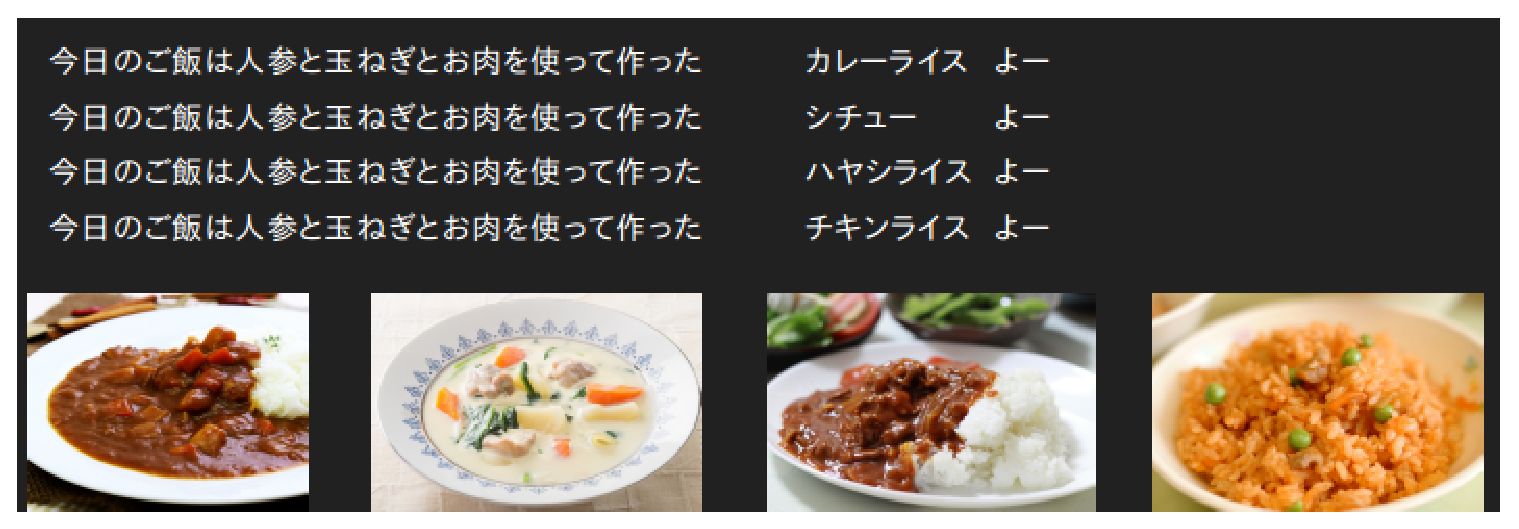
\includegraphics[width=15cm]{../images/kyou_gohan.eps}
  \caption{分布仮設による意味の類推例}
\end{figure}

上述の例は全く同じ文脈で、似たような料理名が出てくる例文を並べたものである。この時、もしどれかひとつの料理名が全く無知なものであったとしても、それが料理であること、どのような料理であるか、ある程度類推することができるだろう。それは、まさしく同じ文脈に出現する単語であるからに違いない。

この考えに則ってベクトルを作成してみる。例えば、
\begin{itemize}
  \item 今日の晩御飯は、ジャガイモの入ったカレーライスだ。
  \item 今日の晩御飯はハヤシライスだ。
\end{itemize}
という二本の文章を例にして、”カレーライス”と”ハヤシライス”の意味表現を考える。

まず、それぞれの文章を形態素解析すると、
\begin{itemize}
  \item $今日 \backslash の \backslash 晩御飯 \backslash は \backslash 、 \backslash ジャガイモ \backslash の \backslash 入っ \backslash た \backslash カレーライス \backslash だ \backslash 。$
  \item $今日 \backslash の \backslash 晩御飯 \backslash は \backslash ハヤシライス \backslash だ \backslash 。$
\end{itemize}
となる(上では $\backslash$ によって形態素を区切っている)。

これをもとに、”カレーライス”と”ハヤシライス”に関して、同じ文脈に着目した意味表現ベクトルを作成する。
同じ文脈に出現する形態素(これ以降文脈語と呼ぶ)をベクトルの各次元とし、注目する単語と何個の同じ文脈でその次元の文脈語が出現しているかを値としてとると、
\begin{itemize}
  \label{weight_equation}
  \item $カレーライス = [(今日:1),(の:1),(晩御飯:1),(は:1),(、:1),(ジャガイモ:1),(入っ:1),(た:1),(だ:1),(。:1)]$
  \item $ハヤシライス = [(今日:1),(の:1),(晩御飯:1),(は:1),(、:0),(ジャガイモ:0),(入っ:0),(た:0),(だ:1),(。:1)]$
\end{itemize}
と表すことができる。\\

ここで、ある単語$x_i$と別な単語$x_j$が何らかの文脈で同時に出現していることを\textbf{共起}していると言い、何度共起しているかの回数を\textbf{共起頻度}と言う。つまり、上記の例で作成したベクトルは、共起頻度を値として持つ\textbf{共起ベクトル}であると言える。\cite{book_wm}この方法でベクトルを作成する場合は、学習に用いられるテキストの集まり(\textbf{コーパス})すべてから学習するため、一般に高次元で疎なベクトルが生成される。これは、コーパスに含まれる単語数が数万程度であったり、単語数に対し、単語同士が共起することは一般に多くないためである。

こうして作成される意味表現ベクトルを用いて別な自然言語処理のタスクを行う際、元々のベクトルが高次元で疎なものであるために、学習事例を正しく表現できなくなってしまうなどの問題が発生してしまう。

\subsection{分散的意味表現}
分布的意味表現ベクトルが高次元で疎なものであるという点を避けた学習方法として提案されたのが、\textbf{分散的意味表現}である。\\
\\
分散的意味表現の学習手法の基本は以下のようになっている。\\
\begin{enumerate}
  \item まず、すべての単語に、任意の固定次元のベクトルを割当て、ランダムな実数値で初期化する。
  \item 与えられたベクトルを用いて、何らかの予測タスクを解く。
  \item 予測タスクを解いた結果に応じてベクトルの値を更新する。
  \item 2へ戻る。
\end{enumerate}

分散的意味表現を表すベクトルの各次元は、何らかの実数値変数が持つ値と解釈することができる。この実数値変数が持つ特徴はどのような予測タスクを解くか、固定次元数をどのくらいの値にするかなどによって変わると予想されるが、単純な共起頻度が値となるわけではなく、また、他の様々な形態素と次元を共有することから、コーパス中で共起することがない形態素同士の関係についても表現しているものと期待されている。

次章では、本研究で用いた形態素の分散的意味表現学習ツールword2vecで実装されている2種類の予測タスクについて述べる。










\chapter*{謝辞}
本研究を進めるにあたって、特別な事情により普通よりも長い期間、丁寧にご指導いただきました原口先生に心から御礼申し上げます。
長い期間の在籍も、研究室内でサポートくださいました大久保先生、配属時の事情など御心配戴きました吉
岡先生にも、厚く御礼申し上げます。

研究を様々な面でサポートしていただきました先輩方、研究室の皆様にも大変お世話になりました。

未熟な私がここまでやってこれたのは、サポートしていただきました皆様のおかげであり、すべての方々に感謝を申し上げます。

\begin{flushright}
  平成二十八年 二月 \\
      平田 泰樹
\end{flushright}


\cleardoublepage



\appendix
\chapter{�����f�[�^}
\label{app_a}

\subsubsection{�f�[�^�P}

\begin{verbatim}
<DOCNO>JA-980814031</DOCNO>
<SECTION>�А�</SECTION>
<WORDS>1298</WORDS>
<HEADLINE>�m�А��n�P�T�J���\�Z�@�낤�����‚΂�܂�����</HEADLINE>
\end{verbatim}

\subsubsection{�f�[�^�Q}
\begin{verbatim}
<DOCNO>JA-980909046</DOCNO>
<SECTION>�А�</SECTION>
<WORDS>1284</WORDS>
<HEADLINE>�m�А��n�ϓ��J���@�L�����E�ɒm�b�����߂�</HEADLINE>
\end{verbatim}

\subsubsection{�f�[�^�R}
\begin{verbatim}
<DOCNO>JA-980924038</DOCNO>
<SECTION>�А�</SECTION>
<WORDS>1278</WORDS>
<HEADLINE>�m�А��n�r�f�I���J�@�ĎЉ�̕ω������Ƃ���</HEADLINE>
\end{verbatim}

\subsubsection{�f�[�^�S}
\begin{verbatim}
<DOCNO>JA-981002046</DOCNO>
<SECTION>�А�</SECTION>
<WORDS>1297</WORDS>
<HEADLINE>�m�А��n�N������@�g�ڋʏ��i�h���̂ċ���̂�</HEADLINE>
\end{verbatim}

\subsubsection{�f�[�^�T}
\begin{verbatim}
<DOCNO>JA-981016042</DOCNO>
<SECTION>�А�</SECTION>
<WORDS>1268</WORDS>
<HEADLINE>�m�А��n���S�–��@�����@���ꂩ��̂ق�����ς�</HEADLINE>
\end{verbatim}

\subsubsection{�f�[�^�U}
\begin{verbatim}
<DOCNO>JA-981021041</DOCNO>
<SECTION>�А�</SECTION>
<WORDS>1232</WORDS>
<HEADLINE>�m�А��n�S�҉�k�@�Ē��̊O��w�͂܂��s��</HEADLINE>
\end{verbatim}

\subsubsection{�f�[�^�V}
\begin{verbatim}
<DOCNO>JA-981023041</DOCNO>
<SECTION>�А�</SECTION>
<WORDS>1296</WORDS>
<HEADLINE>�m�А��n�Q�P���I�֕����x���@�L���Ȓn�����Ă邽��</HEADLINE>
\end{verbatim}

\subsubsection{�f�[�^�W}
\begin{verbatim}
<DOCNO>JA-981106044</DOCNO>
<SECTION>�А�</SECTION>
<WORDS>1259</WORDS>
<HEADLINE>�m�А��n�d�@�{�[�i�X�@�����ѕ���̎��オ����</HEADLINE>
\end{verbatim}

\chapter{クラスタリング結果:例}
\label{app_b}
\section{(北海道,札幌)周辺100単語、5クラスターずつのふりわけ}
\begin{table}[h]
  \begin{minipage}[t]{.45\textwidth}
    \begin{center}
      \caption[]{クラスター内単語数}
      \label{hs100_5}
      \begin{tabular}{|c||c|} \hline
        北海道 & 札幌 \\ \hline \hline
        23 & 28 \\
        29 & 20 \\
        12 & 10 \\
        25 & 22 \\
        11 & 20 \\ \hline
      \end{tabular}
    \end{center}
  \end{minipage}
  \hfill
  \begin{minipage}[t]{.45\textwidth}
    \begin{center}
      \caption[]{クラスターマッチ結果}
      \label{hs100_5match}
      \begin{tabular}{|c||c|} \hline
        北海道 & 札幌 \\ \hline \hline
        0 & 0 \\
        1 & 2 \\
        2 & 1 \\
        3 & 4 \\
        4 & 3 \\ \hline
      \end{tabular}
    \end{center}
  \end{minipage}
\end{table}
\begin{table}[h]
  \center
  \caption{北海道 クラスター内}
  \label{h_100_5}
  \begin{tabular}{|c|c|c|c|c|} \hline
    0 & 1 & 2 & 3 & 4 \\ \hline \hline
    胆振 & 瀬棚郡 & 十勝支庁 & 道内 & 東北地方 \\
    留萌 & 余市町 & 道北 & 札幌 & 九州 \\
    胆振支庁 & 白老町 & 渡島総合振興局 & 十勝 & 青森県 \\
    松前郡 & 仁木町 & 渡島支庁 & 釧路 & 沖縄県 \\
    北海道根室市 & 今金町 & 日高支庁 & 道東 & 東北 \\ \hline
    厚田郡 & 磯谷郡 & 檜山振興局 & 道南 & 秋田県 \\
    積丹半島 & 留寿都村 & 根室支庁 & 札幌市 & 宮城県 \\
    後志 & 上砂川町 & 北空知 & 道外 & 岩手県 \\
    古平町 & 岩内町 & 釧路総合振興局 & 根室 & 鹿児島県 \\
    羅臼町 & 上ノ国町 & 雨竜町 & 釧路市 & 北海道南部 \\ \hline
    爾志郡 & 蘭越町 & 空知支庁 & 空知 & 新潟県 \\
    厚岸町 & 後志支庁 & 檜山支庁 & 函館 &  \\
    八雲町 & 余市郡 &  & 室蘭市 &  \\
    白糠町 & 浦臼町 &  & 小樽 &  \\
    根室市 & 上富良野町 &  & 旭川市 &  \\ \hline
    十勝郡 & 様似町 &  & 道央 &  \\
    寿都郡 & 浦幌町 &  & 旭川 &  \\
    積丹町 & 倶知安町 &  & 稚内市 &  \\
    礼文郡 & 中標津町 &  & 帯広 &  \\
    木古内町 & 広尾郡 &  & 函館市 &  \\ \hline
    幌泉郡 & 増毛町 &  & 苫小牧市 &  \\
    積丹郡 & 芽室町 &  & 網走 &  \\
    乙部町 & 士幌町 &  & 帯広市 &  \\
     & 壮瞥町 &  & 小樽市 &  \\
     & 中札内村 &  & 北海道庁 &  \\ \hline
     & 猿払村 &  &  &  \\
     & 南富良野町 &  &  &  \\
     & 石狩市 &  &  &  \\
     & 留萌市 &  &  &  \\
     &  &  &  &  \\ \hline
  \end{tabular}
\end{table}
\begin{table}[h]
  \center
  \caption{札幌 クラスター内}
  \label{s_100_5}
  \begin{tabular}{|c|c|c|c|c|} \hline
    0 & 1 & 2 & 3 & 4 \\ \hline \hline
    名古屋 & すすきの & 札幌市 & 函館 & 釧路 \\
    北見 & 道内 & 岩見沢 & 小樽 & 室蘭 \\
    十勝 & 帯広市 & 小樽市 & 旭川 & 苫小牧 \\
    金沢 & 稚内 & 北海道札幌市 & 帯広 & 東京 \\
    北海道旭川 & 広島 & 札幌市手稲区 & 北海道 & 大阪 \\ \hline
    長野 & 苫小牧市 & 釧路市 & 仙台 & 北海道札幌 \\
    北見市 & 道東 & 宮の森 & 新潟 & 富山 \\
    岩見沢市 & 空知 & さっぽろ & 旭川市 & 中島公園 \\
    倶知安 & 真駒内 & 札幌西 & 福岡 & 横浜 \\
    神戸 & 登別 & 秋田 & 青森 & 北海道稚内 \\ \hline
    山鼻 & 山形 & 仙台市 & 丘珠 & 札幌中央 \\
    熊本 & 室蘭市 & 岩手 & 江別 &  \\
    北広島市 & 根室 &  & 網走 &  \\
    江別市 & 札幌駅 &  & 函館市 &  \\
    深川市 & 石狩 &  & 盛岡 &  \\ \hline
    札幌市西区 & 札幌市中央区 &  & 留萌 &  \\
    石狩市 & 北海道釧路市 &  & 恵庭 &  \\
    富良野 & 岡山 &  & 新千歳空港 &  \\
    徳島 & 札幌市厚別区 &  & 手稲 &  \\
    北海道美唄市 & 月寒 &  & 琴似 &  \\ \hline
    紋別 & 東北 &  & 千歳空港 &  \\
    鹿児島 & センチュリーロイヤルホテル &  & 丘珠空港 &  \\
    余市 & 北海道名寄市 &  & 北海道旭川市 &  \\
     & 厚別 &  & 千歳市 &  \\
     & 光星高等学校 &  & 北広島 &  \\ \hline
     & 旭川空港 &  &  &  \\
     & 滝川市 &  &  &  \\
     & 東札幌 &  &  &  \\
     & 北海道函館市 &  &  &  \\
     &  &  &  &  \\ \hline
  \end{tabular}
\end{table}



\bibliographystyle{jplain}
\bibliography{skb}

\end{document}
